\section{Quantum Circuits}
\label{sec:circuits}
For this research we have chosen to execute the Teleportation protocol, Grover's
search algorithm, Entanglement Swapping and Entanglement Purification on the
devices. The circuits are all made using an open source software development kit
called Qiskit, which uses Python as its main programming language. The written
codes, made with Jupyter Notebook, for the circuits can be found in the \hyperref[apen]{appendix}. In the following we will describe the circuits,
mainly focussing on the states and the measurements.
Thereafter, a summary of the execution of a code will be given.
\newpage
\subsection{The Teleportation protocol}
\label{sub:tele}
Quantum teleportation is a procedure where a quantum state can be transmitted
from one location to the other. Usually this is done by creating an arbitrary
state $\ket{\psi}$ on the first qubit and a $\ket{\Phi^+}$ Bell-state on the
second and third qubit, as can be seen in figure \ref{fig:telgen}.

\begin{figure}[h]
  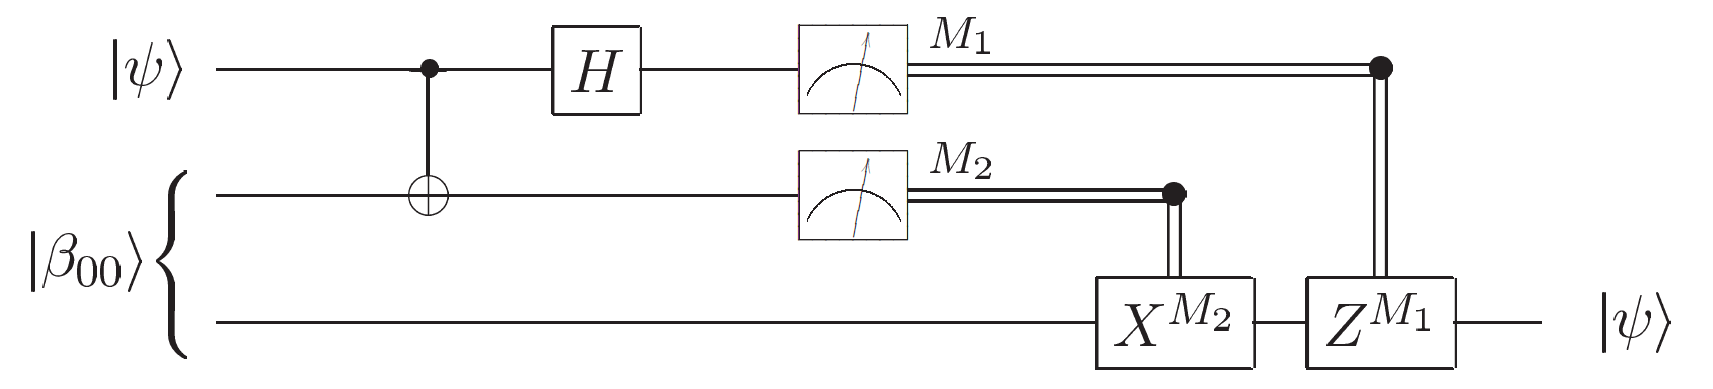
\includegraphics[width=0.48\textwidth]{images/Teleport_general.png}
	\caption{General teleportation protocol circuit. Here the $\ket{\Phi^+}$
Bell-state is denoted as $\ket{\beta_{00}}$. \cite{nielsen10_quant}}
	\label{fig:telgen}
\end{figure}

Subsequently, a CNOT gate is applied to the second qubit and a
Hadamard gate to the first qubit. Now the first and second qubit will be
measured in the Z-basis, with the measurement results being $M_1$ and $M_2$,
respectively. A X- and/or Z-gate is applied to the third qubit depending on the
measurement outcome. If $M_1 = -1$ a Z-gate will be applied and if $M_2 = -1$ a
X-gate will be applied. This will result in the state $\ket{\psi}$ being
teleported to the third qubit.

However, to know if the state $\ket{\psi}$ is properly transported, the third
qubit must be measured. Unfortunately, it is not possible (yet) to apply a gate
after a measurement on the used devices. So, we will have to resort to post
measurement techniques, as the gates cannot be applied to the third qubit. The
circuit that is send to the devices is presented in figure \ref{fig:telcir}.

\begin{figure}[h]
  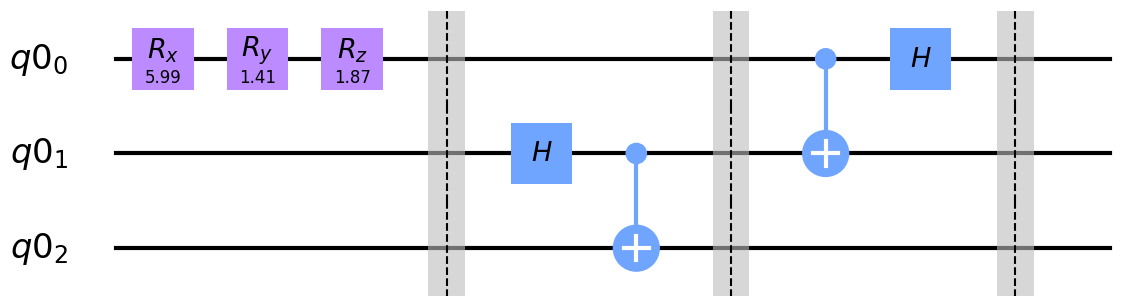
\includegraphics[width=0.48\textwidth]{images/teleport_circuit.png}
	\caption{Teleport circuit used for the measurements. (The operators on the
first qubit are randomized every run.)}
	\label{fig:telcir}
\end{figure}

As one can easily see the gates on the third qubit are absent. To
account for this, a Pauli-X or Pauli-Z matrix is applied to the final state on
the third qubit, after the measurement. Which works similar to the general
protocol: if $M_1 = -1$ a Pauli-Z matrix will be applied and if $M_2 = -1$ a
Pauli-X matrix will be applied. This will, in post measurement, result in the
state $\ket{\psi}$ being teleported to the third qubit.

\subsection{Grover's search algorithm}
The Grover search algorithm can find an input given to a black box with a high
likeliness. In our case, the input that is given is a unitary 4x4 diagonal
matrix, with three values being +1 and one being -1. The algorithm can find
which one of the numbers on the diagonal is -1. The circuit that is used in the
measurements is presented in figure \ref{fig:grocir}.
\begin{figure}[h]
  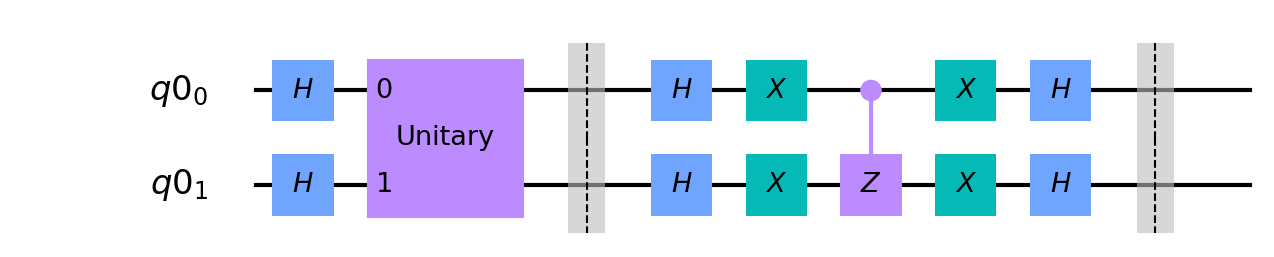
\includegraphics[width=0.48\textwidth]{images/grover_circuit.png}
	\caption{Grover's search algorithm circuit used for the measurements. (The
position of the -1 value is randomized every run.)}
	\label{fig:grocir}
\end{figure}
For explanatory reasons, let us choose the unitary matrix to be:
\begin{equation*} U =
  \begin{bmatrix}
    1 & 0 & 0 & 0 \\
    0 & 1 & 0 & 0 \\
    0 & 0 & 1 & 0 \\
    0 & 0 & 0 &-1
\end{bmatrix}
\end{equation*}
$U$ is randomized for every run of the circuit on a device or
simulator. The two qubit will both start in the $\ket{0}$ state. After the
application of the Hadamard gates the total state will be: $\ket{\Psi} =
\frac{1}{2}\left(\ket{00}+\ket{01}+\ket{10}+\ket{11}\right)$. Now $U$ is applied
giving: $\ket{\Psi} =
\frac{1}{2}\left(\ket{00}+\ket{01}+\ket{10}-\ket{11}\right)$. The part after the
unitary in figure \ref{fig:grocir} is important for the Grover's search
algorithm and does an inversion about the mean. This inverts the constants
multiplied with each state around the mean of the total. In this case the mean
is $\frac{3\cdot\frac{1}{2}-\frac{1}{2}}{4} = \frac{1}{4}$. Inverting
$\frac{1}{2}$ about the mean, means that it will become 0. For $-\frac{1}{2}$ it
will become 1, thus making $\ket{11}$ the only state left. Measuring this will
result in $M_1 = M_2 = -1$. This result is related to where in $U$ the -1 value
is positioned and in this case the result shows it is in the bottom right corner
(where we positioned -1 in the first place).

\subsection{Entanglement swap}
This protocol is, as the name states, a way of changing the entanglement between two qubits, for example the first and second, to an entanglement between different qubits, for example the first and fourth. This circuit will first be generally described, and can be found in figure \ref{fig:swapgen}.
\begin{figure}[h]
	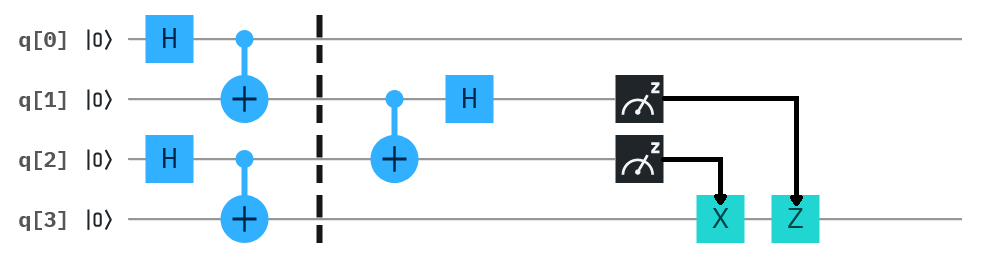
\includegraphics[width=0.48\textwidth]{images/swap_general.png}
	\caption{General entanglement swap protocol circuit. Made using the IBM Quantum experience Circuit Composer.}
	\label{fig:swapgen}
\end{figure}

First, an arbitrary Bell-like state is created on the first two qubits (q[0] and q[1]). For explanatory reasons, this is now a simple $\ket{\Phi^+}$ Bell state. On the third and fourth qubit, a $\ket{\Phi^+}$ state is also created. This gives the following state: $\ket{\Psi} = \frac{1}{2}\left(\ket{0000}+\ket{0011}+\ket{1100}+\ket{1111}\right)$. So at this point our arbitrary state has entanglement with the first and second qubit, which are the fourth and third number in de bra-ket notation, respectively. Now, a CNOT gate is applied between the second and third qubit resulting in: $\ket{\Psi} = \frac{1}{2}\left(\ket{0000}+\ket{0111}+\ket{1100}+\ket{1011}\right)$. After the application of the Hadamard gate to the second qubit we get eight different possible states: 
%Did something weird with the equation here or else it wouldn't fit in the text
$\ket{\Psi} = \frac{1}{\sqrt{8}}(\ket{0000}+\ket{0010}+\ket{0101}-\ket{0111}+\ket{1001}$$-\ket{1011}+\ket{1100}+\ket{1110})$. Now for the measurement part. If the result would be $M_1 = +1$ and $M_2 = -1$, a X-gate is applied to the fourth qubit. This would result in: $\ket{\Psi} = \frac{1}{\sqrt{2}}\left(\ket{0100}+\ket{1101}\right)$. One can see that the first and fourth qubit now have the combined state $\frac{1}{\sqrt{2}}\left(\ket{00}+\ket{11}\right) = \ket{\Phi^+}$, so the entanglement is swapped from the first and the second to the first and the fourth qubit.

However, we have to resort to post measurement techniques. Already stated in the \hyperref[sub:tele]{teleportation protocol} section, gates cannot be applied after
measurement. The circuit that is given to the devices and simulators is shown in
figure \ref{fig:swapcir}.
\begin{figure}[h]
	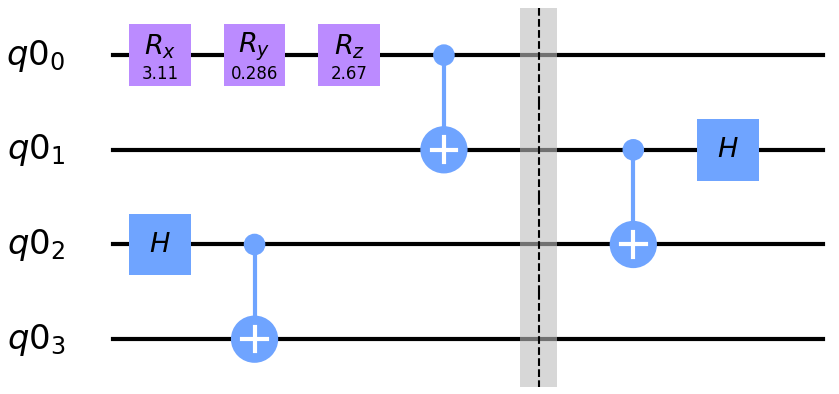
\includegraphics[width=0.48\textwidth]{images/swap_circuit.png}
	\caption{Entanglement swap circuit used in the measurements. Every measurement a random Bell-like state is created on the first two qubits.}
	\label{fig:swapcir}
\end{figure}
At the beginning of every measurement, a random Bell-like state is created. Now, the circuit runs identical to what is explained before, till the measurements take place. After the measurement, a Pauli-X or Pauli-Z matrix is applied to the fourth qubit. This depends on the measurement outcome of $M_1$ and $M_2$. If $M_1 = -1$ we apply a Pauli-Z matrix and if $M_2 = -1$ we apply a Pauli-X matrix. This will give, excluding any errors, an entangled state (post measurement) which we can use for our calculations and comparisons.

\subsection{Entanglement purification}
The entanglement purification is a very useful protocol that ensures a final state is a $\ket{\Phi^+}$ Bell state when the input state is not a perfectly entangled Bell state. This circuit is shown in figure \ref{fig:purcir}. Also, this is the circuit that is used on the devices for measurements.
\begin{figure}[h]
	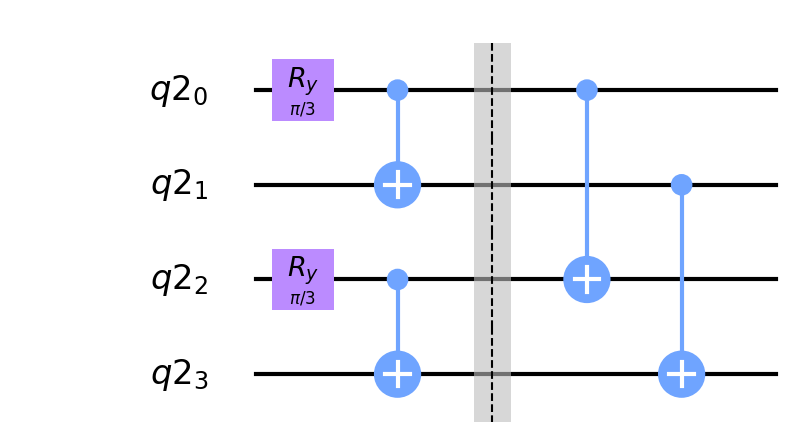
\includegraphics[width=0.45\textwidth]{images/purification_circuit.png}
	\caption{Entanglement purification circuit used in the measurements. The rotation at the beginning of the circuit can be determined using an input fidelity, $F$. In this case $F = 0.75$.}
	\label{fig:purcir}
\end{figure}

First, the circuit makes a not perfectly entangled Bell state by rotating the first and third qubit a certain angle, $\theta$, around the y-axis and subsequently applying a CNOT gate to the first and second and the third and fourth qubit. This angle is determined by a chosen input fidelity, $F$. In this case $F = 0.75$. Later will be explained how this translates to an angle. This will result in the state $\ket{\Psi} = 0.933\ket{0000}+0.067\ket{1111}+0.250\left(\ket{0011}+\ket{1100}\right)$. Now a CNOT gate is applied to the first and third qubit giving: $\ket{\Psi} = 0.933\ket{0000}+0.067\ket{1011}+0.250\left(\ket{0111}+\ket{1100}\right)$. Thereafter, another CNOT gate is applied to the second and fourth qubit: $\ket{\Psi} = 0.933\ket{0000}+0.067\ket{0011}+0.250\left(\ket{1111}+\ket{1100}\right)$. An important part of this circuit is that the bottom two qubit measurements must give -1 as this will ensure that the state of the top two qubits becomes $\ket{\Psi_{1,2}} = \frac{1}{\sqrt{2}}\left(\ket{11}+\ket{00}\right) = \ket{\Phi^+}$. One could argue that a measurement of +1 for both bottom qubits also gives a Bell state, but this state would not have the same factors, so it will not be perfectly entangled. In the measurements we account for this by only fabricating density matrices for the results where the bottom two qubits measurements where -1.

Generally a not perfectly entangled $\ket{\Phi^+}$ state can be described by the following $\ket{\psi} = \cos{\frac{\theta}{2}}\ket{00} + \sin{\frac{\theta}{2}}\ket{11}$, in which $\theta$ is the angle of rotation along the y-axis. The density matrix of this state, $\rho$, can be calculated as 
$\rho = \ket{\psi}\bra{\psi} = \cos^2{\frac{\theta}{2}}\ket{00}\bra{00} + \cos{\frac{\theta}{2}}\sin{\frac{\theta}{2}}\left(\ket{00}\bra{11}+\ket{11}\bra{00}\right)+\sin^2{\frac{\theta}{2}}\ket{11}\bra{11}$. 
The fidelity with respect to the $\ket{\Phi^+}$ state is defined as: $F = \bra{\Phi^+}\rho\ket{\Phi^+}$. Filling in $\rho$ and calculating $F$ will result into $F = \frac{1}{2}\left(1+\sin{\theta}\right)$, which can be rewritten to have $\theta\left(F\right) = \arcsin{\left(2F-1\right)}$. In our case, for $F = 0.75$, the rotation angle $\theta$ would become $\theta = \frac{\pi}{6}$.

\subsection{Code execution}
The circuits are build using Qiskit, a very user friendly open source software that lets the user make quantum circuits and execute them on simulators or devices. IBM their devices are easily implementable in the executions using Qiskit, which gave us the easy choice for using their devices for circuit execution. In the following a concise summary will be given of what steps are taken in the codes for the different circuits. We advise the reader to also have one of our codes visible while reading the summary.

Starting off, the proper modules are imported in the code. One must think about modules for circuit building, visualization, tomography calculations, measurement calibrations, etcetera. Secondly, the IMBQ device needed for the calculation is selected. In order to use the devices, one must have an account at IBM Quantum Experience, where one can get a token which gives (limited) access to their devices. Also, the necessary preparations for the noise calculation are done. As we would like to do a noise simulation using the noise model for the chosen device, this must be properly selected as well. Next, the required circuit is build and visualized, both generally and for the device. An expected state is created from the circuit. This means the state we would expect without any error in the circuit. For the circuits with a Bell-like states, the expected state of the $\ket{\Phi^+}$ is created. This all is done for future fidelity calculation. Subsequently, the measurement readout correction is performed, which is a build in function in Qiskit. This function does a measurement for only certain gates on a empty circuit. Since we are only interested in one or two qubits, we first select which are relevant for our study. For example, the entanglement purification circuit only requires correction on the top two qubits. This is executed on the device 8,192 times (shots). The results are processed accordingly to get the $B$ matrix and $\vec{\beta}$ vector. Next, the tomography circuits are send to the simulator, noise simulator and the device. \newpage These are nine circuits which have a combination of a Hadamard and/or S$^\dagger$-gate before the measurements of the relevant qubits. As before, these have 8,192 shots as well. After the runs, the results are used to make full states in all the possible basis.
 
These full states are then used for the calculation of the density matrices. During this calculation, measurement readout correction and post measurement techniques are also applied. For example, only keeping the data which has $\ket{11}$ as the state for the bottom two qubits in entanglement purification. Using the density matrices acquired from the three runs, the fidelities are calculated by comparing the resulting matrices to the expected one created at the beginning. The execution of the circuits is repeated 15 times, giving a total of 122,880 shots per device.

%%% Local Variables:
%%% mode: latex
%%% TeX-master: "report"
%%% End:
